\chapter{Reference Distance}

This chapter describes the result of the distance measurements for the defined reference data. All calculations and graphs shown in this chapter are produced in the Jupyter Notebook "DistanceReferenceMeasurement.ipynb"

\section{One Hour Reference Time Series}

Due to the rough granularity of one hour both distance measures produce the same result. This is also visualised by the straight diagonal red line in figure \ref{fig:ref_dtw_dist_one_h_granularity}.

\subsection{Euclidean Distance}

The Euclidean Distance between the \ac{hr} time series is: \textbf{0.19867312}


The Euclidean Distance between the \ac{rr} time series is: \textbf{0.31696241}


\subsection{DTW}

The distance using \ac{dtw} between the \acp{hr} values is: \textbf{0.19867312}


The distance using \ac{dtw} between the \acp{hr} values is: \textbf{0.31696241}

\begin{figure}[h!]
	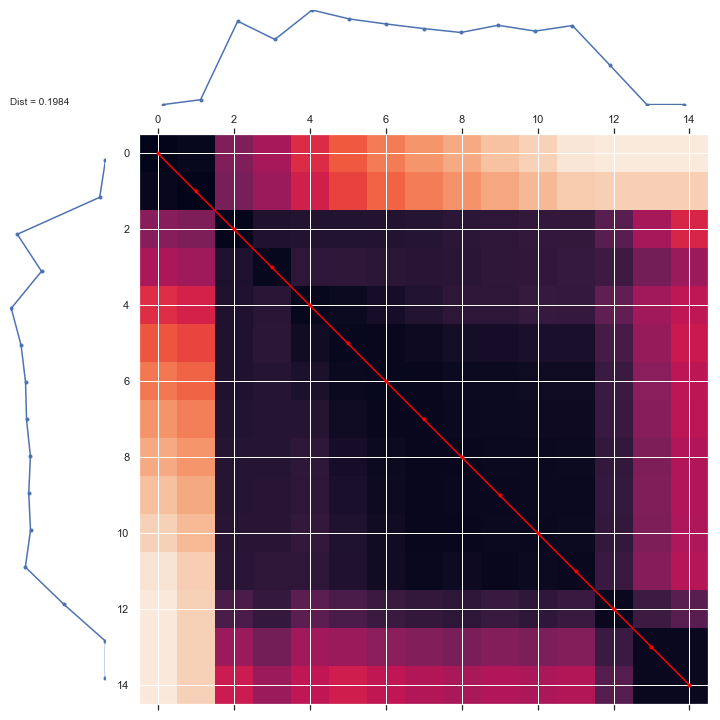
\includegraphics[width=1\textwidth]{ref_1hour_hr_dtw.png}
	\caption{DTW visualisation (HR, 1h granularity)}
	\label{fig:ref_dtw_dist_one_h_granularity}
\end{figure}




\clearpage
\section{30 Minutes Reference Time Series}

Due to the rough granularity of 30min there is no big difference between the Euclidean and \ac{dtw} method.